\subsection{Bus Stop Locations and Routes}
\par This data file contains network information on the location of all bus stops in London, and the sequence of bus stops that every bus route in London stops at. 

\par From this data file, we extracted information on all pairs of neighbouring bus stops and the routes that serve between them. We save this information in the neighbours table in the database. Figure \ref{fig:neighbours_schema} shows the neighbours table scheme. Figure \ref{fig:neighbours_view} shows the sample data stored in neighbours table.

\begin{figure}
\centering
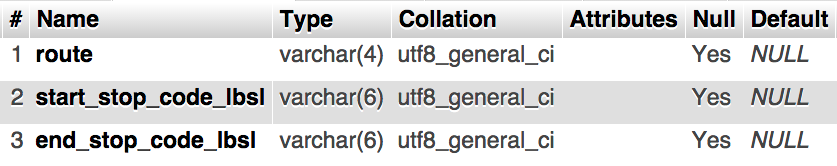
\includegraphics[width=0.9\textwidth]{figures/neighbours_schema.png}
\caption{\label{fig:neighbours_schema} Neighbours table schema}
\end{figure}

\begin{figure}
\centering
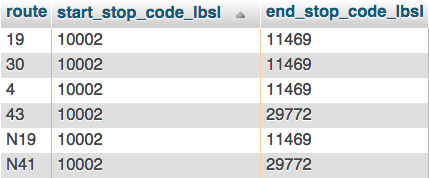
\includegraphics[width=0.7\textwidth]{figures/neighbours_view.png}
\caption{\label{fig:neighbours_view} Data stored in neighbours table}
\end{figure}

\subsubsection{Finding the average travel time between neighbouring stops}
\par To experiment with the queries, we selected one pair of the neighbouring stops (10002, 11469), and listed the time required to travel from stop 10002 to stop 11469 by finding the difference in arrival times for each journey. Sample entries of this list is shown in Figure \ref{fig:journey_time_10002}.

\begin{figure}
\centering
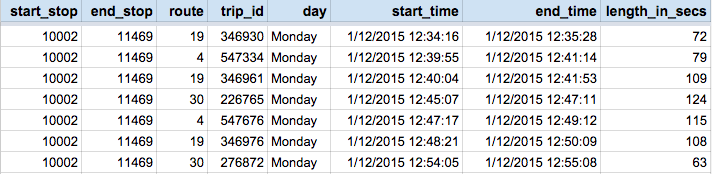
\includegraphics[width=0.7\textwidth]{figures/journey_time_10002.png}
\caption{\label{fig:journey_time_10002} List of journey time from stop 10002 to stop 11469}
\end{figure}


\par We then calculated the average journey time required to travel from 10002 to 11469 for each hour in each week of the day. This information is stored as a timetable, which would be used for further analysis. 

Figure\ref{fig:timetable_10002} shows the timetable generated. Each cell indicates the average journey time required to travel from stop 10002 to stop 11469 at a give hour of a give week of day. The \textbf{NULL} values are due to a current databases performance issue. This will be resolved later.

\begin{figure}
\centering
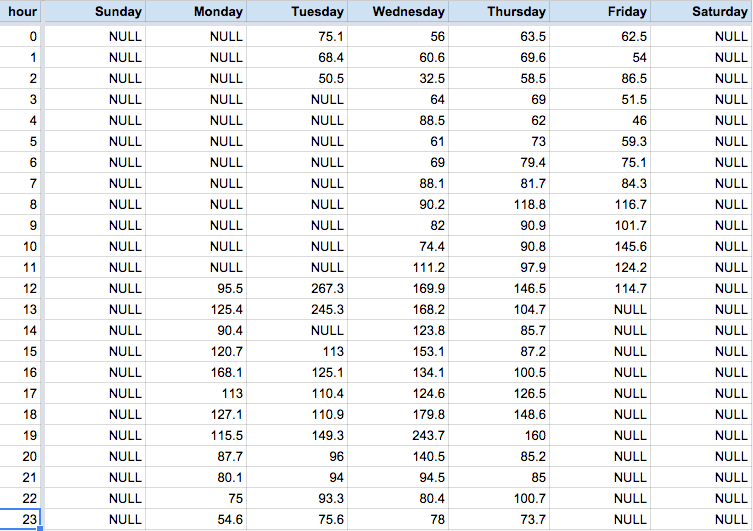
\includegraphics[width=0.9\textwidth]{figures/timetable_10002.png}
\caption{\label{fig:timetable_10002} Average journey time in seconds from stop 10002 to stop 11469 for each hour of each day of week}
\end{figure}

\par We plan to construct a timetable this way for each pair of the neighbouring bus stop.

